% ===== §4 Charting the Ground: Dynamics as Background Manifold =====
\section{Charting the Ground: The Underlying Dynamics as the Background Manifold on which Meaning Unfolds}
\label{sec:dynamics}

\noindent
This chapter differs in kind from an ordinary illustrative chapter. By \xref{sub:gen-hermeneutic}, happiness is hermeneutic, dwells in the symbolic, and the dynamical---a language of the imaginary--real, lacking the symbolic---cannot cross to the dimension of meaning (the demonstration of insufficiency stands). \emph{Yet}, by \xref{sub:gen-manifold}, meaning cannot stand apart from it: the dynamical is the background manifold, the stage, on which meaning unfolds. This chapter therefore has a double office: \emph{(a)~demonstration of insufficiency}---pressing the dynamical vocabulary to its limit, \emph{and showing that the many neighbouring theories which also explain the phenomenon translate into it and stop at the same boundary}, so that ``it cannot cross to the symbolic'' becomes visible at its fullest; and \emph{(b)~bearing}---in doing so, charting the shape of the very ground on which meaning is laid down. The dynamical system here is neither a model of happiness nor a discarded scaffold, but \emph{a ground without meaning yet indispensable}. The breadth of theoretical connection (\xref{sub:dyn-connect}) does not elevate the dynamical to the master account; on the contrary, the wider the web of theories that meet in it, the more decisively their \emph{common} boundary---the failure to reach meaning---is exhibited. Its kinship with \xref{sec:unwritability} is exact: this chapter strains to the utmost to show dynamics insufficient, as the final chapter turns the impossibility of writing into evidence---the same self-referential gesture in formal dress.

\paragraph{Honesty clause.} The toy models below are constructed for illustration; their parameters are not empirically calibrated. They illuminate structure; they prove no empirical fact, and certainly no proposition about happiness (cf.\ \xref{sub:gen-methodology}, \xref{sub:gen-hermeneutic}).

\subsection{What this chapter guards against}
\label{sub:dyn-guard}

The downgrading is restated, with one warning peculiar to this chapter. By the foregoing chapters, ``happiness $=$ a fixed form'' is already foreclosed; what this chapter must guard against is its last hiding-place---the equation of \emph{some preferred dynamical property} (asymptotic stability, ergodicity, the capacity to escape) with happiness. The chapter will show that dynamics is \emph{neutral} as to ``what happiness is,'' and that the cause of the neutrality is the lack of the symbolic (\xref{sub:gen-hermeneutic}). The point is made with equations, so that both the neutrality and the lack come into view.

\subsection{An arraying of candidate properties: each dynamical property courts an intuition of happiness}
\label{sub:dyn-array}

\paragraph{The harmonic oscillator (the base).} Let each subject be an oscillator. The \emph{linear} oscillator, $\ddot{x}+\omega^{2}x=0$, has closed circular orbits---but it is \emph{neutrally stable} (no basin of attraction; perturb it and it merely switches to another orbit). This answers to a ``happiness of chance'': resembling happiness, yet dispersed by a single push. Already visible: the plainest ``stability'' will not bear the intuition of happiness.

\paragraph{The limit cycle (van der Pol).} Add nonlinear damping:
\begin{equation}
\ddot{x}-\varepsilon\,(1-x^{2})\,\dot{x}+\omega^{2}x=0 .
\end{equation}
At small amplitude the damping is negative (energy injected), at large amplitude positive (energy dissipated); the system converges to a \emph{unique, asymptotically stable limit cycle}---neither decaying to rest nor diverging, oscillating perpetually and returning to itself after perturbation (Figure~\ref{fig:limitcycle}). This answers to a ``rhythmic abiding happiness.'' (As a side-image of ``the gap lived in the mode of fullness'': energy-injection $\approx$ the real's continual regeneration of the gap, dissipation $\approx$ continual symbolisation, the cycle $=$ the gap not vanishing while the system never stops. The gap appears here only as a damping metaphor; an explicit gap-dimension is not unfolded.)

\begin{figure}[t]
\centering
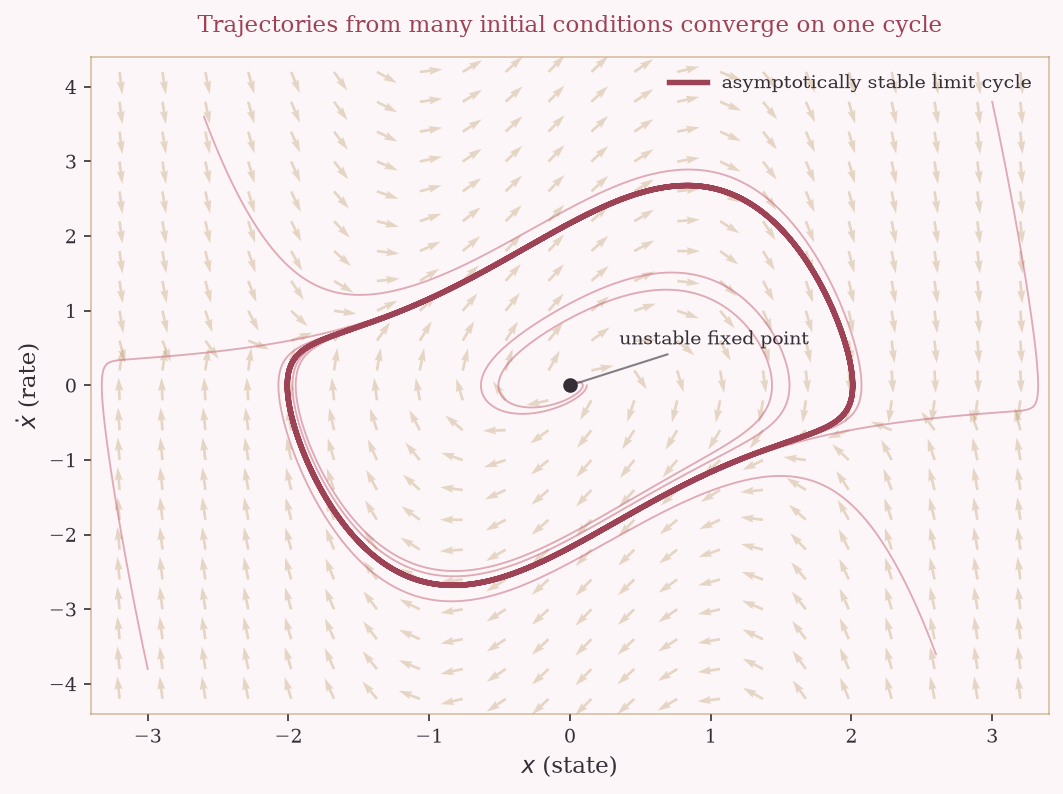
\includegraphics[width=0.82\linewidth]{figures/limit_cycle.png}
\caption{Trajectories from many distinct initial conditions---inside and outside---spiral onto one asymptotically stable limit cycle (deep rose). The origin is an unstable fixed point. The cycle has a \emph{basin of attraction}: after a perturbation the system returns to it. This is a side-image of the abiding mode, charting one region of the manifold's shape---\emph{not} a definition of happiness.}
\label{fig:limitcycle}
\end{figure}

\paragraph{Basin of attraction and asymptotic stability.} These answer to the ``abiding'' intuition: predictably stable, returning after perturbation---the \emph{stability party}'s happiness.

\paragraph{Multiple attractors and metastable switching.} Where the phase space holds several attractors and the system can switch among them (metastability), the answer is the ``exploration'' intuition: able to go somewhere new, not locked in---the \emph{novelty party}'s happiness.

\paragraph{Edge-of-chaos / strange attractors.} High-dimensional trajectories, never repeating yet always bounded, answer to a ``creative'' happiness---each day different yet always within a form of life (the mode left as a thread in \xref{sub:modes-open}, here a legitimate candidate piece).

\paragraph{The capacity to escape a basin.} Not stability itself but the capacity to \emph{leave} the current basin answers to a ``freedom'' intuition.

Each candidate has its equations, each is self-consistent, each can be claimed by some intuition of happiness.

\subsection{Dynamics as a lingua franca: how the same phenomenon is explained by, and connects to, other theories}
\label{sub:dyn-connect}

The objection must now be met that \emph{other theories also explain the phenomenon}---predictive coding, synchronisation theory, thermodynamics, cybernetics, catastrophe theory, the geometric-phase account of Paper~IX. This is true, and it is not a weakness of the dynamical illustration but its deepest point: the vocabulary of dynamical systems is a \emph{lingua franca} into which these otherwise disparate theories can be translated, and which therefore exhibits both their connection \emph{and}---the load-bearing turn---the single boundary they all share. The wider the web of translation, the more decisively the boundary shows: \emph{every one of these is a language of the manifold, and none reaches conferral of meaning} (\xref{sub:gen-hermeneutic}). Breadth of connection serves subordination, exactly as in \xref{sec:neuro}.

\paragraph{Limit cycle $\leftrightarrow$ predictive coding / free energy.} A stable attractor is, in the predictive-coding register, a low-free-energy state \citep{friston2010}; the system's settling onto the cycle is its minimisation of long-run prediction error. The translation is exact---and both languages, equally, lack the symbolic: a low-free-energy state no more ``means'' contentment than a stable orbit does (\xref{sub:neuro-fullness}).

\paragraph{Coupled oscillators $\leftrightarrow$ Paper XVIII's phase capture.} Two coupled oscillators, in the Kuramoto register \citep{kuramoto1984,strogatz2001}, synchronise by mutual frequency entrainment; this is the very mathematics of Paper~XVIII \citep{paperxvii}, where unilateral capture is pathological (one party's autonomous term overwhelmed) and bilateral co-rotation is healthy. The dynamical illustration of \xref{sub:coex-waiting} and the relational claim of \xref{sec:coexistence} thus share one formal object---and the difference between capture and co-rotation, recall, is adjudicated not within the mathematics but at the symbolic level (whether the place of conferral is preserved).

\paragraph{Basin of attraction $\leftrightarrow$ cybernetics, homeostasis, allostasis.} Return to an attractor after perturbation is, in the cybernetic register, negative-feedback regulation \citep{wiener1948}; in the physiological register, homeostasis, and---predictively---allostasis, stability through anticipated change \citep{sterling2012}. This connects the ``robustness'' of happiness (\xref{sec:coexistence}, and Paper~XVII's generative balance versus static equality \citep{paperxvii}) to a wide family of regulation theories. All describe the \emph{return}; none says what the return \emph{means}.

\paragraph{Non-equilibrium steady state $\leftrightarrow$ dissipative structures.} The plain happiness is \emph{still} on the surface yet \emph{generating} beneath---a description that maps precisely onto a \emph{dissipative structure}, a non-equilibrium steady state maintained by continual flux \citep{prigogine1984}. This is perhaps the sharpest formal side-image of ``uneventful yet generating'': macroscopically stable, microscopically never at rest. It connects the present account to the thermodynamics of self-organisation---and, once more, the thermodynamic description carries no meaning: a dissipative structure is not, as such, happy.

\paragraph{Geometric phase / holonomy $\leftrightarrow$ Paper IX's good cycle.} The geometric phase (Berry phase) accumulated around a closed loop \citep{berry1984} is the formal criterion Paper~IX \citep{paperix} used for the good cycle: a return that is transformed rather than mere reversion, a spiral rather than a circle. Here the dynamical illustration connects directly to the series' founding formalism---the limit cycle's ``return that is not mere repetition'' is the holonomy of Paper~IX in another coordinate.

\paragraph{Bifurcation / catastrophe $\leftrightarrow$ the transition between modes.} The shift between the mode of lack and the mode of fullness (\xref{sub:gen-twomodes}) is, formally, a change of attractor under a varying parameter---a bifurcation, in catastrophe-theoretic terms a phase change \citep{thom1975,haken1983}. The qualitative suddenness of a shift from drivenness to dwelling has a formal name.

\begin{table}[t]
\caption{Dynamics as lingua franca: each neighbouring theory explains a facet of the phenomenon, connects to a dynamical concept, and shares the one boundary---none reaches conferral of meaning (\xref{sub:gen-hermeneutic}).}
\label{tab:dyn-connect}
\small
\begin{tabularx}{\linewidth}{>{\RaggedRight\arraybackslash}p{3.0cm} >{\RaggedRight\arraybackslash}p{3.2cm} >{\RaggedRight\arraybackslash}X}
\toprule
\textbf{Theory} & \textbf{Dynamical connection} & \textbf{Facet explained / shared boundary} \\
\midrule
Predictive coding / free energy & Stable attractor $=$ low-free-energy state & Plainness as low error; cannot mean contentment by itself \\
Kuramoto synchronisation & Coupled oscillators; entrainment & Shared rhythm; capture vs co-rotation (Paper XVIII) \\
Cybernetics / allostasis & Basin of attraction $=$ feedback regulation & Robustness, return after perturbation; not its meaning \\
Dissipative structures & Non-equilibrium steady state & ``Still yet generating''; not, as such, happy \\
Geometric phase / holonomy & Closed-loop transformed return & Good cycle (Paper IX); spiral not circle \\
Catastrophe / synergetics & Bifurcation between attractors & Transition: mode of lack $\leftrightarrow$ mode of fullness \\
\bottomrule
\end{tabularx}
\end{table}

\paragraph{The lesson of the web.} These six translations show that the dynamical vocabulary connects a remarkable range of theories that each explain a facet of the plain happiness. But the very success of the translation is what carries the argument: \emph{all six are languages of the manifold, and the rightmost column of Table~\ref{tab:dyn-connect} records, in every row, the same failure to cross into meaning.} That so many theories converge here, and that all stop at the same boundary, is far stronger evidence for \xref{sub:gen-hermeneutic} than the limit cycle alone could give. The breadth is the proof.

\subsection{The conflict: these properties cannot be jointly maximised}
\label{sub:dyn-conflict}

The decisive fact: the candidates stand in \emph{real tension, statable with equations}. Sharpest: \emph{asymptotic stability (return to the original orbit after perturbation) and attractor-escape (the capacity to reach a new attractor) are mathematically opposed}---the deeper the basin, the more stable, the harder to escape; the more readily switching and exploratory, the less stable. One cannot jointly maximise ``returning'' and ``getting elsewhere.'' The stability party and the novelty party do not misunderstand one another; they have \emph{preferred opposed properties of the phase space}. Both are right, both have equations. This is precisely the demonstration of \xref{sub:gen-hermeneutic}: dynamics can formalise every intuition of happiness, and \emph{cannot adjudicate among them}.

\subsection{Non-adjudicability: no meta-criterion within dynamics selects ``which property is happiness''}
\label{sub:dyn-nonadjudicate}

\emph{Within} the language of dynamics there is no higher dynamical quantity that judges ``asymptotic stability is more happy than ergodicity'' or the reverse. Any such judgement has already imported a value, a conferral of meaning, from \emph{outside}. The cause (per \xref{sub:gen-hermeneutic}): adjudication belongs to the \emph{symbolic} (conferral of meaning); dynamics, lacking the symbolic, \emph{cannot reach it}---not informational insufficiency, but the wrong register. Here the ``boundary'' shows itself: dynamics, pressed to its fullest (every candidate arrayed, every tension made explicit), reveals at exactly that point the line it can never cross.

\subsection{Rejoining \xref{sec:generativity} and \xref{sub:modes-open}: how the open thesis stands ``above'' these properties}
\label{sub:dyn-rejoin}

The open thesis of \xref{sec:generativity} (rhythmed by self-continuation, operating in the mode of fullness, exhausted by no single form) does \emph{not} take the side of the stability party or the novelty party: it neither requires resting in a stable cycle (``not settling itself'' would exclude that), nor requires perpetual leaping to the new (that is merely another pinned-down preference). It stands \emph{above} stability and novelty, and so can hold both as modes under differing material-historical conditions. This formally redeems \xref{sub:modes-open}: the array of \emph{mutually conflicting} candidate properties is the concrete unfolding of that chapter's ``left-open ellipsis,'' and their \emph{non-adjudicability} is the formal proof that the ellipsis must be left open. Openness is no longer only a philosophical posture; it receives, on the manifold, a witness: the non-adjudicability is the complexity of the terrain on which meaning must unfold, a terrain that does not choose for meaning.

\subsection{Closing: the ground is laid, happiness unfolds upon it}
\label{sub:dyn-close}

The chapter does not end in failure. It has, with equations, exhausted what dynamics can say, and thereby confirmed two things: \emph{(a)~demonstration of insufficiency}---this language does not reach the meaning of happiness (meaning is in the symbolic); \emph{(b)~bearing}---it has thereby charted the shape of the background manifold on which meaning unfolds (\xref{sub:gen-manifold}). Dynamics is thus \emph{a ground without meaning yet indispensable}: meaning is not in it, but meaning cannot stand apart from it. It is neither abolished nor elevated---it sets the stage, and happiness, as meaning, unfolds upon it, mediated by the symbolic order. The form here returns the meaning to philosophy and remains, itself, the ground of meaning, not its sovereign.
